\documentclass[11pt]{article}
\usepackage[margin=1in]{geometry}
\usepackage{amsmath,amssymb}
\usepackage{booktabs}
\usepackage{multirow}
\usepackage{graphicx}
\usepackage[colorlinks=true,linkcolor=blue,citecolor=blue,urlcolor=blue]{hyperref}
\usepackage{xcolor}
\usepackage{microtype}
\usepackage{tikz}
\usetikzlibrary{arrows.meta,positioning,fit,backgrounds,calc}

\definecolor{frozengray}{HTML}{6B7280}
\definecolor{trainedblue}{HTML}{2563EB}
\definecolor{geogreen}{HTML}{059669}
\definecolor{froz}{HTML}{F3F4F6}
\definecolor{trai}{HTML}{DBEAFE}
\definecolor{geob}{HTML}{D1FAE5}

\newcommand{\metric}{AP$_{50}^{\text{axis+origin}}$}
\newcommand{\apfifty}{AP$_{50}$}

\title{Geometry Beats Regression:\\
A Diagnosis-Driven, Almost-Training-Free Recipe for\\
Scene-Level Articulated Part Understanding}

\author{
  Junyuan Fang\\
  \texttt{fangjunyuan1@gmail.com}
  % TODO: affiliations, co-authors
}
\date{August 2026}

\begin{document}
\maketitle

\begin{abstract}
We describe our solution to the Articulate3D challenge (OpenSUN3D, ECCV
2026). The task: find every movable part in a real-world 3D indoor scan and
predict how it moves --- rotation or translation, the motion axis, and the
axis origin. Our entries placed first on both dev leaderboards and second
on both test leaderboards of the challenge's two tasks. On the movable-part
task we improve the official USDNet baseline from test \metric{} $=0.264$
to $\mathbf{0.4056}$ ($+54\%$ relative). On the companion interactable-part
task we improve from $0.2686$ to $\mathbf{0.3286}$ ($+22\%$).

The recipe combines a few components that can be read independently:
\begin{itemize}
\item \textbf{Diagnosis before design.} Per-instance error forensics shows
  the two articulation heads fail for different reasons: the axis head
  collapses onto the dominant gravity-aligned mode, and the origin head
  shrinks predictions toward the part centroid.
\item \textbf{Training-free geometric priors} replace the learned
  regressors: translation axes read off the panel geometry of the predicted
  mask, rotation origins snapped to a mask endpoint on the side opposite the
  predicted handle, and rotation axes forced vertical. This takes the test
  score from $0.264$ to $0.3385$ with the segmentation branch bit-identical.
\item \textbf{One trained component}: an $88$K-parameter attention-pooled
  origin head, finetuned with every other parameter frozen ---
  \emph{including} BatchNorm running statistics.
\item \textbf{Structural post-processing}: the model routinely merges the
  two leaves of a double door into one instance. Splitting predicted masks
  into spatially connected components (DBSCAN) transfers near-fully to
  test, lifting the movable task to $0.3760$ and the interaction
  task from $0.2686$ to $0.2886$.
\item \textbf{A bet against a memorized validation set}: the released
  checkpoints were trained on train$+$validation, so validation scores them
  in-sample. A mirror-flip finetune gained only $+0.004$ on validation but
  $+0.027$ on test, and an equal-strength two-model ensemble reached
  $0.3240$. Transplanting the same recipe to the movable model on deadline
  day delivered the final $0.4056$ and $0.3286$.
\end{itemize}

We also document more than two dozen negative results, including two silent
training pitfalls: frozen parameters do not stop BatchNorm buffers from
drifting, and finetuning a released checkpoint can restart its coarse-to-fine
curriculum from scratch. This report is iterative competition engineering
under a one-submission-per-day budget, not a set of controlled ablations; we
flag every comparison that is confounded.
\end{abstract}

\section{Introduction}

Articulated part understanding asks a model to find every movable part in a
scene-level 3D scan and to predict how it moves: the motion type (rotation or
translation), the motion axis, and --- for rotations --- the origin of that
axis. The Articulate3D benchmark~\cite{halacheva2025articulate3d} poses this
task on 280 high-fidelity ScanNet++~\cite{yeshwanth2023scannetpp} indoor
scans, with the USDNet baseline built on
Mask3D~\cite{schult2023mask3d}/MinkowskiNet~\cite{choy2019minkowski}.

Our starting point is a faithful reproduction of the USDNet baseline
(test \metric{} $=0.2640$, matching the officially published $0.26$). We do
not scale the model or the training. Instead we follow a strict
\emph{diagnosis-first} methodology: measure exactly where the metric loses
points, attribute each loss to a mechanism in the pipeline, and prefer the
cheapest intervention --- ideally a training-free geometric one --- that
addresses that mechanism.

Five observations shaped everything that follows. The first three arrived in
the opening weeks; the last two only in the campaign's final days.

\begin{enumerate}
\item \textbf{Segmentation is not the bottleneck.} Our mask \apfifty{}
  ($0.437$) already led the public leaderboard. The deficit relative to the
  leading entry was entirely in \emph{articulation retention} --- the fraction
  of correctly segmented instances that also pass the axis and origin
  criteria ($65\%$ for us vs.\ $77\%$ for the leader at the time).
\item \textbf{The two articulation heads fail differently.} Axis errors are
  bimodal: a large correct mode plus a $90^\circ$ failure mode. Origin errors
  are unimodal but systematically biased. A single fix cannot address both.
\item \textbf{Scene geometry already contains most of the answer.} Doors and
  drawers are planar, hinges live on part boundaries, and handles sit
  opposite hinges. Reading these facts off the predicted masks outperforms
  the learned regressors that were trained to approximate them.
\item \textbf{Instance merging is a structural defect, and structural fixes
  transfer.} The model routinely merges the two leaves of a double door (or
  two adjacent handles) into one instance, corrupting every geometric
  quantity computed on the merged mask.
  Splitting masks into spatially connected components is
  distribution-independent --- ``two doors are two objects'' is true on any
  split --- and, unlike our tuned thresholds, its gains transferred near-fully
  to test (\S\ref{sec:structural}).
\item \textbf{A memorized validation set hides exactly the gains that
  matter.} The released checkpoints were trained on train$+$validation, so
  validation scores them in-sample. A finetune with mirror-flip augmentation
  moved validation by $+0.004$ and test by $+0.027$: the augmentation
  dividend was nearly invisible on the memorized split
  (\S\ref{sec:extension}). When quota permits, arbitration must be held out.
\end{enumerate}

\section{Related Work}

\textbf{Scene-level articulation.} Articulate3D~\cite{halacheva2025articulate3d}
extends part-level articulation prediction from object-centric datasets to
full ScanNet++ scenes. Its reference method is USDNet: a Mask3D-style
transformer instance segmenter with added MLP heads that regress a
3-vector axis and origin per query.

\textbf{Canonicalized articulation estimation.}
ANCSH~\cite{li2020ancsh} showed that predicting joint parameters in a
normalized canonical space outperforms direct regression in camera space.
RPMArt~\cite{wang2024rpmart} votes joint parameters from point tuples for
robustness. Our PCA-normal and endpoint priors follow the same philosophy ---
express the target in a frame the part itself defines --- but require no
training at all.

\textbf{Test-time geometric reasoning.} Our priors can be seen as a
deterministic, interpretable post-process, in contrast to learned refinement
stages. They leave the segmentation branch untouched by construction.

\section{Preliminaries}

This section fixes the task, the metric, and the data. It also states
exactly which organizer-provided artifacts we consumed --- a point that
matters later, because two of them were trained on the validation split.

\subsection{Task and metric}

For each scene the submission provides $N$ instances, each with a point mask,
a confidence, a class $c \in \{\text{rotation}, \text{translation}\}$, an
axis $\mathbf{a} \in \mathbb{R}^3$ and an origin $\mathbf{o} \in
\mathbb{R}^3$. The leaderboard metric --- we call it the \emph{joint metric}
and write it \metric{}; the toolkit calls it \texttt{MAO\_ST} --- counts a
prediction as true positive iff
\begin{align}
\text{IoU}(\text{mask}) &> 0.5, \qquad
\arccos\!\left(|\cos(\mathbf{a}, \mathbf{a}^{gt})|\right) < 15^\circ,\\
\big\|P_{\mathbf{a}^{gt}}^{\perp}(\mathbf{o}-\mathbf{o}^{gt})\big\| &< 0.25\,\text{m}
\;\;\wedge\;\;
\big\|P_{\mathbf{a}}^{\perp}(\mathbf{o}-\mathbf{o}^{gt})\big\| < 0.25\,\text{m},
\end{align}
where $P^{\perp}$ projects out the component along an axis; translation
instances skip the origin test.

Three properties matter in practice. First, the axis test is
\emph{sign-agnostic}. Second, origin correctness is a \emph{point-to-line}
distance, so sliding an origin along the axis is free. Third, the
evaluator's projection divides by $\|\mathbf{a}\|$ rather than
$\|\mathbf{a}\|^2$, so predicted axes must be normalized --- an implementation
detail worth $+0.018$ \metric{} on validation by itself.

\subsection{Data: what the organizers provide, and what we consumed}
\label{sec:data}

Everything in this paper runs on organizer-provided artifacts; we used no
external data. The Articulate3D annotations cover 279 ScanNet++ v1 indoor
scenes with 6349 articulations (4687 rotation, 1662 translation). They
comprise: movable-part instance masks with per-part articulation parameters
(type, axis, origin) for the main task; interaction-element instance masks
(handles, knobs, buttons) for the companion task; and a USD scene-hierarchy
annotation, which we did not use. The official split is 195 train / 42
validation / 42 test scenes. Test labels are withheld and scored only by the
challenge server. The organizers additionally release preprocessed point
clouds (the mesh downsampled at a $1$\,cm voxel size; evaluation runs on
$2$\,cm-voxelized clouds carrying the ground truth) and two USDNet
checkpoints, \texttt{mov\_trainval.ckpt} and \texttt{inter\_trainval.ckpt}.
Both checkpoints were trained on train$+$validation --- a fact that matters
twice in what follows.

How each piece was used, concretely:
\begin{itemize}
\item \textbf{train (195 scenes):} the only data our early head finetune
  (the $88$K origin attention head, \S\ref{sec:originhead}) trained on.
\item \textbf{train$+$validation (237 scenes):} what the released
  checkpoints saw --- the root of the validation-memorization effect we
  later exploited (\S\ref{sec:extension}) --- and what our augmented
  finetunes \texttt{v5}/\texttt{v6}/\texttt{mov\_v11} retrain on.
\item \textbf{validation (42 scenes):} our offline arbiter. We rebuilt the
  official evaluation to bit-exactness against the challenge server
  (verified on two submissions), so all iteration ran offline without
  spending submission quota. Every diagnosis statistic in this paper ---
  error forensics, oracle ceilings, cue inventories --- is measured here.
\item \textbf{test (42 scenes):} points only, no labels. Every test number
  in this paper is a server-returned score of a numbered submission.
\item \textbf{Cross-task coupling:} predicted interaction masks are an
  \emph{input} to the movable task via the hinge-opposite-handle rule
  (\S\ref{sec:geo}). Companion-task quality therefore propagates into
  main-task origins, which \S\ref{sec:structural} exploits deliberately.
\item \textbf{Per-scene arrays:} all offline post-processing, including the
  DBSCAN splitting of \S\ref{sec:structural}, consumes only the preprocessed
  per-scene \texttt{.npy} arrays (xyz, RGB, normals, semantic and instance
  ids) --- no meshes, no images, no re-inference.
\end{itemize}
Not used: the ScanNet++ RGB streams (DSLR or iPhone), meshes beyond the
preprocessed clouds, the USD hierarchy/connectivity annotations, and any
external data. Omitting the image modality is not merely convenient: our cue
inventory (\S\ref{sec:selection}) measured that RGB and normals --- the two
input columns the pipeline never consumed --- carry no hinge signal.

\subsection{Baseline}

USDNet predicts articulation from the transformer queries: per-point features
inside each predicted mask are \emph{mean-pooled} and decoded by MLPs into
axis and origin (its ``mode 2''). We reproduce the released checkpoint at
test \metric{} $=0.2640$.

\section{Diagnosis}
\label{sec:diagnosis}

Before changing anything, we measure where the baseline loses points. The
two heads fail through different, identifiable mechanisms, which licenses
fixing them separately.

We match predictions to ground truth on the validation split
(greedy, IoU $>0.5$; 275 matched instances) and analyze the two heads
separately. Our harness reproduces the official validation numbers
bit-for-bit (and matched the challenge server on a probe submission), so
all analysis is against the exact deployed metric.

\begin{figure}[t]
\centering
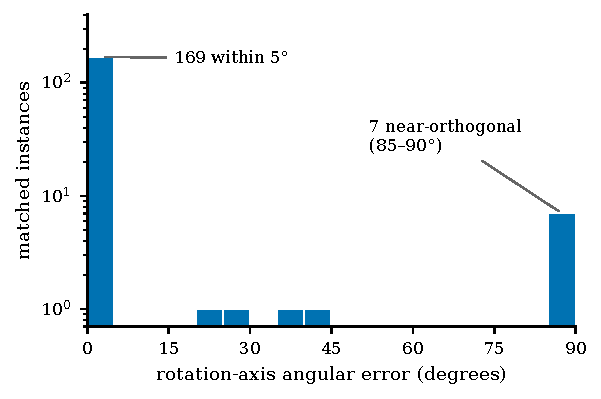
\includegraphics{figs/fig_axis_error_hist}
\caption{\textbf{Baseline rotation-axis errors} (log-$y$; $n=180$ matched
validation rotations): $169$ instances fall within $5^\circ$ (median
$2.7^\circ$), while the $7$ lateral hinges all fail at $85$--$90^\circ$ ---
the head outputs $\approx(0,0,1)$ regardless of the part.}
\label{fig:axishist}
\end{figure}

\textbf{Axis: mode collapse onto gravity.}
$93.3\%$ of matched rotation axes in GT are vertical within $15^\circ$, and
the regression head, trained with a $1-\cos$ loss on this distribution,
collapses onto that mode: every lateral hinge (oven/dishwasher-style) fails
at $85$--$90^\circ$ (Figure~\ref{fig:axishist}). Strikingly, the trivial
rule ``always predict gravity'' passes $93.3\%$ of rotation axes vs.\ the
model's $88.3\%$ (0 wins / 9 losses for the model). The learned head's
entire value lies in translation azimuths, where gravity is always wrong.

\textbf{Origin: centroid shrinkage from mean aggregation.}
Rotation-origin error is unimodal (median $0.127$\,m against a $0.25$\,m
threshold) with no global offset: an oracle global translation improves the
pass rate by only $+0.006$. The real bias is \emph{shrinkage}. $77\%$ of
predicted origins are displaced from the GT hinge toward the part centroid,
recovering only $29\%$ of the centroid-to-hinge distance. The mechanism is
architectural: mode-2 aggregation averages (offset $+$ coordinate) over
\emph{all} mask points, and a mean over a door pulls any estimate toward the
middle of the door, while hinges live on its edge. Consistently, an oracle
that snaps origins to mask endpoints given GT axes recovers the hinge for
$100\%$ of instances (median residual $8$\,mm), while the centroid passes
only $28\%$.

\textbf{Independence.} Axis and origin failures are nearly independent
($\phi=-0.11$), so fixes compose additively.

\section{Method}

\begin{figure*}[t]
\centering
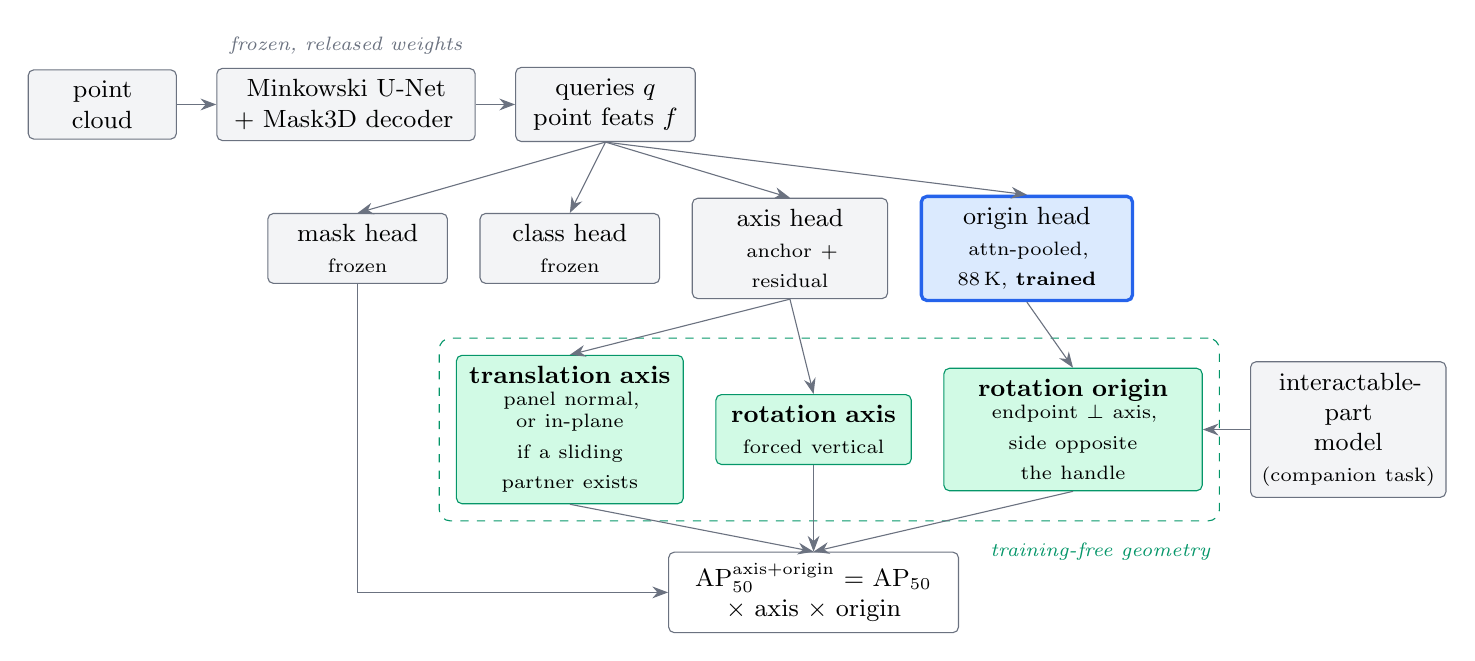
\begin{tikzpicture}[
  font=\small,
  box/.style={draw, rounded corners=2pt, align=center, inner sep=4pt,
              minimum height=8mm, text width=#1},
  froznode/.style={box=#1, fill=froz, draw=frozengray},
  trainode/.style={box=#1, fill=trai, draw=trainedblue, very thick},
  geonode/.style={box=#1, fill=geob, draw=geogreen},
  ar/.style={-{Stealth[length=2mm]}, draw=frozengray},
  lbl/.style={font=\scriptsize\itshape, text=frozengray},
]

% ---- row 1: input and backbone ----
\node[froznode=16mm] (pc) {point\\cloud};
\node[froznode=30mm, right=5mm of pc] (bb)
  {Minkowski U-Net\\ $+$ Mask3D decoder};
\node[froznode=20mm, right=5mm of bb] (feat) {queries $q$\\ point feats $f$};

\draw[ar] (pc) -- (bb);
\draw[ar] (bb) -- (feat);
\node[lbl, above=0.5mm of bb] {frozen, released weights};

% ---- row 2: heads ----
\node[froznode=20mm, below left=9mm and 20mm of feat.south] (mh) {mask head\\\scriptsize frozen};
\node[froznode=20mm, right=4mm of mh] (ch) {class head\\\scriptsize frozen};
\node[froznode=22mm, right=4mm of ch] (ah) {axis head\\\scriptsize anchor $+$ residual};
\node[trainode=24mm, right=4mm of ah] (oh) {origin head\\\scriptsize attn-pooled, 88\,K, \textbf{trained}};

\foreach \n in {mh,ch,ah,oh} \draw[ar] (feat.south) -- (\n.north);

% ---- row 3: training-free geometry ----
\node[geonode=26mm, below=9mm of ch] (gtr)
  {\textbf{translation axis}\\\scriptsize panel normal, or in-plane\\\scriptsize if a sliding partner exists};
\node[geonode=22mm, right=4mm of gtr] (grot)
  {\textbf{rotation axis}\\\scriptsize forced vertical};
\node[geonode=30mm, right=4mm of grot] (gor)
  {\textbf{rotation origin}\\\scriptsize endpoint $\perp$ axis,\\\scriptsize side opposite the handle};

\draw[ar] (ah.south) -- (gtr.north);
\draw[ar] (ah.south) -- (grot.north);
\draw[ar] (oh.south) -- (gor.north);

% handles come from the companion task; kept to the right of the origin rule
% so the arrow does not have to cross the other two geometry boxes
\node[froznode=22mm, right=6mm of gor] (hnd)
  {interactable-part\\model\\\scriptsize (companion task)};
\draw[ar] (hnd.west) -- (gor.east);

\begin{scope}[on background layer]
  \node[fit=(gtr)(grot)(gor), draw=geogreen, dashed, rounded corners,
        inner sep=6pt] (geobox) {};
\end{scope}
\node[lbl, text=geogreen, anchor=north east]
  at ([yshift=-1.5mm]geobox.south east) {training-free geometry};

% ---- row 4: outputs ----
\node[box=34mm, below=11mm of grot, draw=frozengray, fill=white] (out)
  {\metric{} $=$ \apfifty{} $\times$ axis $\times$ origin};
\draw[ar] (gtr.south) -- (out.north);
\draw[ar] (grot.south) -- (out.north);
\draw[ar] (gor.south) -- (out.north);
% masks bypass the geometry entirely -- routed below the dashed box
\draw[ar] (mh.south) |- (out.west);

\end{tikzpicture}
\caption{\textbf{The recipe.} Everything on the mask pathway is frozen at the
released weights, so \apfifty{} is bit-identical to the baseline by
construction. Exactly one component is trained --- an $88$\,K-parameter
attention-pooled origin head, with BatchNorm statistics pinned
(\S\ref{sec:freeze}). The articulation parameters that the metric actually
scores are then \emph{overwritten} by training-free geometry read off the
predicted mask: the axis head's own output survives only as the anchor prior
inside the dashed box. Handle masks for the hinge-side rule come from the
challenge's companion interactable-part task.}
\label{fig:pipeline}
\end{figure*}

This section describes the pipeline (Figure~\ref{fig:pipeline}). The design
follows directly from the diagnosis: keep the segmentation frozen, train one
small origin head, and overwrite the articulation parameters with geometry
read off the predicted masks.

\subsection{Freezing discipline: keep what already works}
\label{sec:freeze}

Because segmentation led the leaderboard, our first design rule is that the
mask pathway must remain \emph{bit-identical}. Freezing parameters
(\texttt{requires\_grad=False}) is \textbf{not sufficient}: BatchNorm running
statistics are buffers, refreshed by any forward pass in training mode. In an
early experiment all 124 BN buffers drifted while every non-articulation
parameter stayed frozen, which changed the masks and manufactured a
$+0.015$ validation ``gain'' that vanished when the statistics were
restored (Table~\ref{tab:bn}). We therefore
pin every \texttt{\_BatchNorm} module to \texttt{eval()} for the whole run,
re-applied each epoch, since the trainer resets module modes.

\begin{table}[t]
\centering
\small
\begin{tabular}{lcccc}
\toprule
Checkpoint (same weights) & \apfifty{} & AP$_{50}^{\text{axis}}$ & AP$_{50}^{\text{origin}}$ & \metric{} \\
\midrule
baseline                     & 0.5711 & 0.4419 & 0.4495 & 0.3215 \\
$+$ head, BN \emph{drifted}  & 0.5720 & 0.4558 & 0.4513 & 0.3369 \\
$+$ head, BN \emph{restored} & 0.5711 & 0.4419 & 0.4486 & 0.3215 \\
\bottomrule
\end{tabular}
\caption{\textbf{BatchNorm-drift confound (validation).} A 4-epoch trained
origin head appears to help ($+0.015$) --- until the drifted BN buffers are
restored to the source checkpoint, revealing the head itself contributed
nothing. All 124 BN buffers had moved; all frozen parameters were
bit-identical.}
\label{tab:bn}
\end{table}

\subsection{The one trained component: attention-pooled origins}
\label{sec:originhead}

We replace the mean over mask points with a learned attention pooling:
$88$K parameters, a scoring MLP plus the original origin MLP. It trains with
everything else frozen as in \S\ref{sec:freeze}, so any change in \metric{}
is attributable to the aggregation alone. Training uses the metric-aligned
point-to-line loss and a sign-agnostic $1-|\cos|$ axis loss --- the metric
takes $|\cos|$, and penalizing a $180^\circ$ flip with maximum loss fights
the evaluator. The head trains on the 195 train scenes only. The released
baseline was trained on train$+$val, which silently inflates its validation
scores by $\sim$$0.01$; this is worth knowing when comparing numbers.

\subsection{Axis anchors instead of free regression}

Following the bimodality in \S\ref{sec:diagnosis}, the axis is expressed as a
choice between two \emph{anchors}: gravity $\mathbf{z}$, and the free
regression axis flattened into the horizontal plane. We keep the regressed
azimuth rather than quantizing it; a fixed azimuth grid measurably loses
($0.449$/$0.466$/$0.468$ AP$_{50}^{\text{axis}}$ for $\{z{+}4\}$/$\{z{+}8\}$
azimuths/ours). With zero-initialized selection and residual layers the
module \emph{exactly} reproduces ``snap to the nearest anchor'' at load time.
That alone is worth $+0.024$ AP$_{50}^{\text{axis}}$ on validation with no
training.

\subsection{Training-free geometric priors}
\label{sec:geo}

This subsection gives the three rules that overwrite the learned
articulation outputs --- translation axis, rotation origin, hinge side ---
each targeting one mechanism from \S\ref{sec:diagnosis}.

\textbf{(i) Translation axis from panel geometry.} Sliding parts are planar,
and the panel's own geometry localises the slide direction far better than
the network does. The smallest-PCA direction of the predicted mask's points,
flattened to the horizontal plane, has median azimuth error $0.70^\circ$ on
matched validation translations; the axis head's is $5.54^\circ$. We adopt
the PCA direction whenever it agrees with the model's axis within
$25^\circ$; the agreement gate protects non-planar parts. Because the metric
skips the origin test for translations, this directly lifts the translation
half of \metric{}.

A planar panel admits \emph{two} horizontal slide directions, however, and
assuming the normal is a statement about drawers only. A sliding door or
window leaf travels \emph{along} its own face, so its axis is the in-plane
horizontal --- exactly $90^\circ$ from the normal. Nine matched validation
translations are of this kind, and the rule above gets every one of them
maximally wrong. The model cannot arbitrate: having learnt a
drawers-slide-outward prior, its axis lies closer to the normal on all of
them.

We therefore decide the question geometrically, from the partner a sliding
leaf must have. Two leaves sit in \emph{different} planes about one leaf
thickness apart, so that one can pass behind the other, and they stand
beside each other at matching height. A row or stack of drawers shares one
plane exactly, and coplanar fronts cannot pass each other. Concretely, a
translation part is flipped to its in-plane direction when another predicted
translation panel is parallel within $20^\circ$, offset through the plane by
$0.004$--$0.06$\,m, displaced laterally, overlapping in height, and itself
planar and of matching height. On validation the plane offset separates the
two classes without overlap: the in-plane cases sit at $0.008$--$0.035$\,m,
the drawer-like ones at $0.000$, $0.089$, $0.245$, $1.30$ and $1.84$\,m.

One further condition is invisible on validation: a sliding leaf must be
door-sized. A row of drawer fronts is also same-height and near-coplanar,
so the pair test alone accepts it, and on the test split the rule was
rotating $0.23$\,m and $0.33$\,m panels --- one of them the highest-scoring
prediction in its scene --- until we added a $0.45$\,m floor on leaf
height. Every true in-plane case on validation is at least $0.50$\,m tall,
so the floor leaves the validation score bit-identical. A validation sweep
cannot discover this kind of condition: the split simply contains no
counterexample.

The rule's validation gain does not transfer in proportion, and the reason
is visible before submitting: it fires $91$ times on the $41$ validation
scenes but only $35$ times on the $42$ test scenes, because eight of its
nine validation positives come from one wardrobe. The $+0.021$ it earns
there measures how much sliding furniture that split contains.
Plateau-checking guards against a threshold being fitted to the data;
nothing guards against the \emph{phenomenon} being concentrated in it.

Requiring the partner to be planar and height-matched --- rather than testing
only whether the part itself is flat --- is what makes this safe. The
one-sided version peaks higher at a planarity threshold of $0.05$ but falls
\emph{below} the no-flip baseline at $0.03$ and $0.08$; eight of its nine
positives come from a single validation scene, so it is fitted to one piece
of furniture. Stating the pair symmetrically flattens the surface: with a
height tolerance of $0.15$, every planarity threshold from $0.03$ to $0.35$
improves \metric{}, by between $+0.004$ and $+0.021$.

\textbf{(ii) Rotation origin $=$ perpendicular endpoint.} We snap each
rotation origin to one of the two robust ($5/95\%$ quantile) endpoints of the
mask along its widest direction \emph{perpendicular to the predicted axis}.
The perpendicularity is essential. A door's longest direction is vertical,
and snapping along the first PCA direction moves origins to the top/bottom
edge, costing $-0.19$ AP$_{50}^{\text{origin}}$; the correct construction
recovers $+0.014$.

\textbf{(iii) Hinge side $=$ opposite the handle.} Which of the two endpoints
carries the hinge? Doors open away from their handles. We reuse the
challenge's companion task: the interactable-part model predicts handle
masks, and if a predicted handle lies near the part, we choose the endpoint
\emph{farther} from it, falling back to the endpoint nearest the predicted
origin otherwise. On matched validation rotations this raises the origin
pass rate from $78.3\%$ to $82.8\%$. Notably it picks the ``correct side''
slightly \emph{less} often ($86.1\%$ vs.\ $88.9\%$): its mistakes
concentrate on parts where both endpoints fail anyway, while its wins occur
where the choice matters.

\section{Experiments}

This section reports the main results, then four studies of the deployed
pipeline: a re-diagnosis, a confounded submission and its controlled
replacement, the remaining bottleneck, and the negative results.

\subsection{Setup}
Articulate3D challenge splits: 195 train / 42 val / 42 test scenes.
All validation numbers use the official evaluator; our local harness matches
the challenge server bit-for-bit (verified on two submissions). Inference is
nondeterministic (unseeded); repeated runs vary by $\pm 0.002$, which we
treat as the noise floor.

The backbone, decoder and mask head are the released USDNet weights
throughout, so \apfifty{} is constant across post-processing changes
\emph{within} a checkpoint. It is not constant across checkpoints. Our
train$+$val origin retrain leaves the predicted masks byte-identical but
alters \texttt{pred\_classes} and \texttt{pred\_scores}; because average
precision depends on the confidence ranking and the per-class grouping,
measured \apfifty{} moves from $0.4370$ to $0.4366$. We flag this because we
initially assumed otherwise and reported a carried-over \apfifty{} for the
retrained rows.

\subsection{Main results}

\begin{table}[t]
\centering
\small
\begin{tabular}{lcccc}
\toprule
Configuration (cumulative) & \apfifty{} & AP$_{50}^{\text{axis}}$ & AP$_{50}^{\text{origin}}$ & \metric{} \\
\midrule
\multicolumn{5}{l}{\emph{Validation}}\\
USDNet baseline (reproduced)          & 0.5711 & 0.4419 & 0.4495 & 0.3215 \\
$+$ trained origin attention          & 0.5711 & 0.4419 & 0.4717 & 0.3477 \\
$+$ axis anchors (warm start)          & 0.5716 & 0.4677 & 0.4717 & 0.3743 \\
$+$ PCA panel normal (\S\ref{sec:geo}.i)   & 0.5716 & 0.4836 & 0.4717 & 0.4049 \\
$+$ endpoint $+$ handle side (\S\ref{sec:geo}.ii--iii) & 0.5716 & 0.4836 & 0.4926 & 0.4306 \\
$+$ swept endpoint quantile \& handle margin (\S\ref{sec:sweep}) & 0.5716 & 0.4836 & 0.5018 & 0.4395 \\
$+$ sliding-leaf axis flip (\S\ref{sec:geo}.i) & 0.5716 & 0.5046 & 0.5018 & 0.4605 \\
$+$ rotation axes forced vertical & 0.5716 & 0.5063 & 0.5018 & 0.4621 \\
$+$ DBSCAN structural split (\S\ref{sec:structural}) & 0.5801 & --- & 0.5393 & 0.5021 \\
$+$ cleaned handle source (\S\ref{sec:structural}) & 0.5801 & --- & 0.5411 & \textbf{0.5038} \\
\midrule
\multicolumn{5}{l}{\emph{Test (challenge server)}}\\
USDNet baseline (reproduced)          & 0.4370 & 0.3801 & 0.3160 & 0.2640 \\
val-fitted post-processing only       & 0.4370 & 0.3887 & 0.3254 & 0.2834 \\
full recipe                           & 0.4370 & 0.4060 & 0.3601 & 0.3345 \\
\quad $+$ train$+$val origin retrain (2 runs) & --- & --- & 0.357 & 0.331--0.332 \\
\quad \quad $+$ sliding-leaf flip (confounded, \S\ref{sec:confound}) & 0.4366 & 0.4051 & 0.3578 & 0.3322 \\
$+$ leaf flip $+$ vertical rotation axes & 0.4370 & 0.4101 & 0.3601 & 0.3385 \\
$+$ DBSCAN structural split (\S\ref{sec:structural}) & 0.4444 & 0.4105 & 0.3955 & 0.3689 \\
\textbf{$+$ cleaned handle source (best pre-extension)} & \textbf{0.4444} & 0.4105 & \textbf{0.4026} & \textbf{0.3760} \\
\midrule
Leaderboard leader (concurrent, pre-extension) & 0.4352 & \textbf{0.4135} & 0.3547 & 0.3360 \\
Runner-up (pre-extension board)       & --- & --- & --- & 0.3393 \\
\bottomrule
\end{tabular}
\caption{\textbf{Main results.} All rows above the DBSCAN split keep the
segmentation branch frozen; \apfifty{} is constant \emph{within} a checkpoint,
but not across them (the train$+$val retrain leaves masks byte-identical while
altering \texttt{pred\_classes} and \texttt{pred\_scores}, which moves
\apfifty{} to $0.4366$). The leaf-flip row stood first on the ranking metric
at the time, ahead of the concurrent leader by $0.0024$; it differs from the
\emph{full recipe} row only in translation and rotation axes --- \apfifty{}
and AP$_{50}^{\text{origin}}$ return bit-identical to seven decimals, so its
$+0.0041$ axis gain is attributable to those two rules alone
(\S\ref{sec:confound}). The DBSCAN structural split is the single deliberate
mask-touching operation of the campaign (\S\ref{sec:structural}); the
cleaned-handle row is our best pre-extension score, $0.0367$ ahead of the
pre-extension runner-up. The deadline-day retrain that supersedes it
appears in \S\ref{sec:extension} and Table~\ref{tab:final}. Validation
axis sub-metrics for the split rows were not re-measured in isolation
(---).}
\label{tab:main}
\end{table}

\begin{figure}[t]
\centering
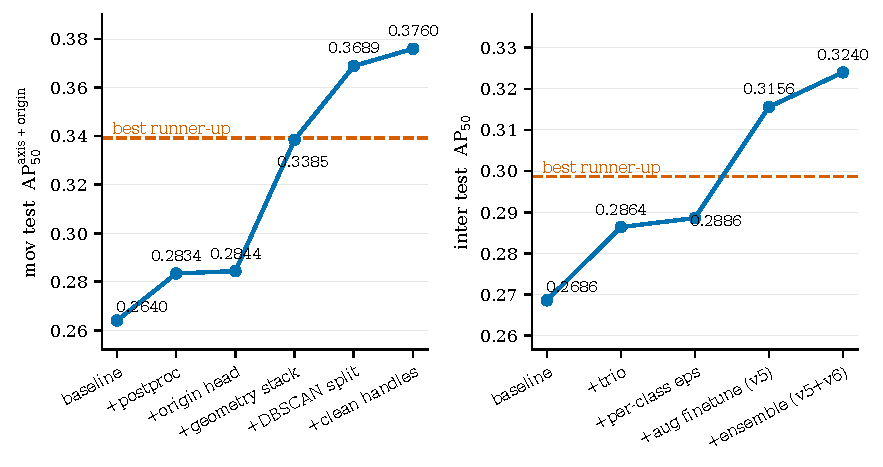
\includegraphics[width=\textwidth]{figs/fig_test_progression}
\caption{\textbf{Official test-score trajectories}; every point is a
server-returned score. Left, movable task: $0.2640$ (baseline)
$\to 0.3385$ (geometric recipe) $\to 0.3689$ (DBSCAN split) $\to 0.3760$
(cleaned handle source). Right, interaction task: $0.2686 \to 0.2886$
(per-class trio) $\to 0.3156$ (\texttt{v5} finetune) $\to 0.3240$
(ensemble). Dashed lines mark the best visible competitor at the original
deadline ($0.3393$ and $0.2904$). A deadline-day retrain later raised our
final scores to $0.4056$/$0.3286$ (\S\ref{sec:extension}).}
\label{fig:progression}
\end{figure}

\begin{figure}[t]
\centering
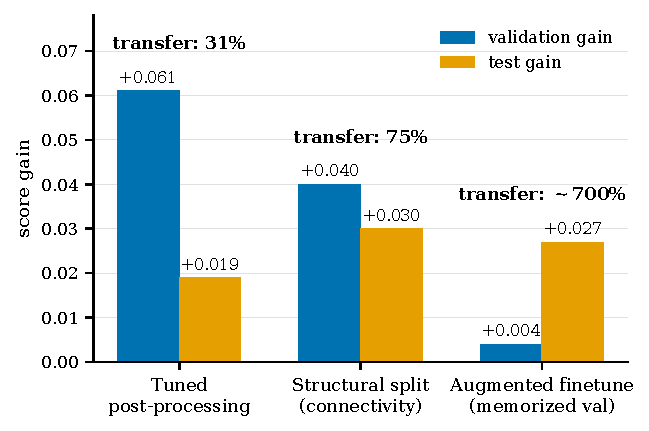
\includegraphics{figs/fig_val_test_transfer}
\caption{\textbf{Validation gain vs.\ realised test gain, by kind of
change.} Tuned thresholds keep $31\%$ of their validation gain on test; the
structural DBSCAN split keeps $75\%$; the mirror-flip finetune realises
$\sim$$700\%$, because a memorized validation set cannot see the
generalization that augmentation buys.}
\label{fig:transfer}
\end{figure}

Table~\ref{tab:main} summarizes the progression;
Figure~\ref{fig:progression} traces the server-verified trajectories on
both tasks. Figure~\ref{fig:transfer} shows the pattern that organised the
campaign: how much of a validation gain reaches test depends on the
\emph{kind} of change. Validation-tuned thresholds transferred at roughly
$1{:}3$ --- double optimism from fitted hyperparameters plus a validation
set the released backbone had trained on. The geometric recipe transferred
at $\sim$$1.2{:}1$ (val $+0.042 \rightarrow$ test $+0.049$): panel normals
and hinge-opposite-handle are properties of the world, not of the split.

A third regime is neither of these. The sliding-leaf rule is
parameter-robust and physically correct, yet transferred at only $1{:}5.5$
(val $+0.0227 \rightarrow$ test $+0.0041$), because the phenomenon it fires
on is concentrated in the validation split (\S\ref{sec:geo}). A rule's
\emph{firing count on the target split} is observable before submitting and
predicts the realised gain far better than its validation gain does; we
recommend reporting it.

\subsection{Re-diagnosing the deployed pipeline}
\label{sec:sweep}

Every diagnosis in \S\ref{sec:diagnosis} was run on \emph{baseline}
predictions. Once the geometric priors rewrite every axis and every
rotation origin, the error profile is a different distribution. We
initially failed to re-measure it, and spent considerable effort on lateral
hinges (7 instances, proven unfixable) while the actual residual sat
elsewhere. Re-running the per-instance breakdown on the deployed stack:

\begin{center}
\small
\begin{tabular}{lccc}
\toprule
& axis pass & origin pass & both \\
\midrule
rotation ($n{=}180$) & 93.3\% & 83.3\% & 80.6\% \\
translation ($n{=}95$) & 91.6\% & --- & 91.6\% \\
\bottomrule
\end{tabular}
\end{center}

Rotation failures decompose as 5 axis-only, \textbf{23 origin-only}, 7 both.
After the geometric axis work, origin dominates the residual by $4.6\times$.
Six instances sit within $1.5\times$ of a threshold: two translation axes at
$15.2^\circ/16.8^\circ$, and four origins at $0.306$--$0.340$\,m.

That points at two hand-picked constants never swept. The endpoint quantile
is strongly unimodal with a broad plateau, and the handle-ownership margin
is monotone:

\begin{center}
\small
\begin{tabular}{lcccccccc}
\toprule
quantile & 2/98 & 5/95 & \textbf{10/90} & 12/88 & 15/85 & 20/80 & 25/75 & 30/70 \\
\metric{} & .4187 & .4306 & \textbf{.4359} & .4354 & .4345 & .4292 & .3810 & .3027 \\
\midrule
handle margin (m) & 0.10 & 0.15 & 0.25 & 0.35 & 0.50 & & & \\
\metric{} & \textbf{.4395} & \textbf{.4395} & .4359 & .4359 & .4330 & & & \\
\bottomrule
\end{tabular}
\end{center}

Both curves are plateaus rather than spikes, which is the criterion we used
to accept them. The mechanisms are interpretable: past the $\sim$20th
percentile the ``endpoint'' is no longer an endpoint (hence the collapse),
and a generous ownership margin lets a \emph{neighbouring} part's handle
vote and flip the hinge side. Two further constants swept in the same run
--- the canonical-snap cone ($15^\circ$--$45^\circ$) and the handle score cut
($0.3$--$0.7$) --- are completely flat, i.e.\ saturated. Together these lift
validation $0.4306 \rightarrow 0.4395$.

\subsection{A confounded submission, and the controlled one that replaced it}
\label{sec:confound}

We first packaged the sliding-leaf rule on top of a different checkpoint
than our best submission used, changing the base and the post-processing at
once. The server returned $0.3322$ against a standing best of $0.3345$,
which reads as the rule having hurt. It had not: that checkpoint's own
baseline scored $0.331$--$0.332$, so the rule was flat-to-positive and the
loss came from the base. The two changes were unseparable after the fact,
and the submission slot was wasted.

We then re-packaged the rule as a \emph{minimal edit}: the identical
prediction file with only translation axes rewritten. This made the next
result readable, and let us state a falsifiable prediction beforehand ---
\apfifty{} and AP$_{50}^{\text{origin}}$ must come back bit-identical. They
did, to seven decimal places ($0.4369668$ and $0.3601476$), while
AP$_{50}^{\text{axis}}$ rose by $0.0041007$ and \metric{} by $0.0039516$.
That number is the two axis rules' contribution with nothing else mixed in.
The resulting submission stood first on the ranking metric at the time:
$0.33845$ against the previous leader's $0.33601$.

The discipline generalises: when submissions are scarce, change one thing
and predict an invariant that must survive it --- the invariant tells you
the measurement is clean before you interpret it.

\subsection{The remaining bottleneck is selection, not representation}
\label{sec:selection}

This subsection asks what limits the deployed pipeline: the origin is the
weak factor, the correct point is always present in the mask, and no
available signal selects it better than the handle rule already does.

Pushing past our submitted score means improving one of the three factors in
\metric{} $\approx$ \apfifty{} $\times\, r_{\text{axis}} \times r_{\text{origin}}$,
which on test read $0.4370 \times 93.85\% \times 82.42\%$. The arithmetic
points somewhere counter-intuitive. Making the axis \emph{perfect} yields
only $0.360$; making the origin perfect yields $0.410$. Origin, not axis, is
the weak factor --- and we had spent our effort on the axis.

Origin turns out not to be limited by segmentation at all. For every matched
rotation the predicted mask \emph{contains} a point within $0.25$\,m of the
ground-truth axis line, median $6$\,mm: the mask ceiling is $100\%$. Against
that, the deployed rule scores $85.0\%$, the best of its two endpoint
candidates $88.3\%$, and a widened family sweeping quantile and depth
$95.6\%$. The answer is present and we cannot select it.

We then asked which signal could. We treat the hinge \emph{edge} as the
single latent that determines both quantities: the axis runs along it, and
the origin lies on it. For each available cue we measured its own AUC for
``is this the hinge edge'', sampling along the whole edge rather than in a
ball around one endpoint:

\begin{center}
\small
\begin{tabular}{lcc}
\toprule
signal & AUC & individual accuracy \\
\midrule
handle distance & \textbf{0.820} ($12.2\sigma$) & \textbf{90.4\%} \\
emptiness beyond the edge & 0.567 ($2.0\sigma$) & 57.1\% \\
normal crease at the edge & 0.519 & 53.8\% \\
colour difference across the edge & 0.493 & 48.7\% \\
contact with static geometry & 0.449 & 37.8\% \\
colour variance along the edge & 0.435 & 35.9\% \\
\bottomrule
\end{tabular}
\end{center}

RGB and the surface normals --- the two inputs the pipeline had never used ---
carry nothing. The handle is the only informative cue, and it is already
deployed. This also explains a failure we had found puzzling: a logistic
selector over these features, under leave-one-scene-out CV, scores $78.9\%$,
\emph{below} the hand-written rule, because it dilutes the one real signal
with five noisy ones.

Finally we asked whether the network's own representation knows better than
our hand-crafted cues --- the question behind ``train a new head rather than
retrain the backbone''. We probe the $256$-d input to the anchor module
(query embedding concatenated with mask-pooled point features) over $137$
instances, leave-one-scene-out, against a permutation null. Predicting where
along its width the hinge sits gives $R^2 = -0.301$ against a null of
$-0.213 \pm 0.115$, i.e.\ $0.8\sigma$ --- no signal. With a frozen backbone a
new head can only exploit what the features already contain, and the hinge
location is not in them.

This corrects our own earlier reasoning: we had leaned for days on a probe
with only \emph{seven} positives --- far too few for an AUC to establish
absence. The properly powered experiment agrees with it, but only the
latter is evidence.

\subsection{Negative results}
\label{sec:negative}

Table~\ref{tab:negative} lists every failed attempt of the campaign, one
row each, including those of the extension window (\S\ref{sec:extension}).
Each consumed real experiment time and shaped the final recipe. Four
failures carry a mechanism instructive beyond their row; they get short
postmortems below.

\begin{table}[t]
\centering
\footnotesize
\begin{tabular}{@{}p{0.27\textwidth}p{0.40\textwidth}p{0.27\textwidth}@{}}
\toprule
Attempt & Outcome & Root cause \\
\midrule
\multicolumn{3}{@{}l}{\emph{Main campaign}}\\
joint training, $3\times$ oversampling $+$ $5\times$ loss weighting &
  \metric{} $0.374 \to 0.089$ in 4 epochs &
  rebalanced $13{:}1 \to \approx 1.4{:}1$; arg-max selector mass-flips
  (postmortem) \\
bounded residual on anchored axes ($\leq 5.7^\circ$, residual-only
  trainable) &
  $+0.004$ raw; stacked $0.4219$ vs $0.4306$ &
  gain absorbed by the PCA prior \\
wide-flat $\Rightarrow$ lateral-hinge classifier &
  precision $8\%$ &
  lateral parts include small box-like lids \\
unconditional panel normal (agreement gate dropped) &
  retention $91.6\% \to 96.8\%$, yet AP$_{50}^{\text{axis}}$ $-0.010$ &
  retention ignores the low-confidence tail (postmortem) \\
model arbitrates the two slide directions &
  wrong on $5$ of $5$ in-plane cases &
  the drawer prior is the bias being corrected \\
stacking detector for lateral hinges &
  holds for $0$ of the $7$ lateral parts &
  appliance doors do not stack as assumed \\
obstruction detector for lateral hinges &
  occupancy $0.213$ vs $0.157$; $3$ of $7$ have nothing above &
  premise false in this data \\
superpoint mask snapping (3 variants) &
  \apfifty{} $0.5716 \to 0.5699/0.5697/0.5665$ (repair);
  $0.5122$ fine / $0.2254$ coarse rebuild &
  semantic vs.\ geometric boundaries (postmortem) \\
learned origin-side selector (\S\ref{sec:selection}) &
  $78.9\%$ vs the rule's $85.0\%$; $1.7\sigma$ from null &
  dilutes the one real signal \\
widened origin candidate family &
  $10/90$ stays optimal; face offset $+0.6$ pts (noise); all three side
  selectors exactly $85.0\%$ &
  face-side sign is a cross product, not physics \\
seed-ensemble TTA &
  runs differ $\pm 0.002$; $97\%$ shared instances, median best-IoU $1.0$ &
  no usable diversity \\
mirror-flip TTA (3 fusion variants) &
  best variant $0.4292$ vs the $0.4306$ single-pass stack &
  mirrored scenes are OOD for the backbone (postmortem) \\
anchor classifier for lateral hinges &
  $+0.0002$ \metric{} in 12 epochs &
  temperature-$10$ warm start: $\sim$$10$-logit wall, gradients
  $\mathcal{O}(10^{-5})$ \\
``flat-lying panels hinge laterally'' rule &
  fires on 3 parts, breaks 2; lone true lateral $90^\circ \to 58^\circ$ &
  still a miss \\
``hinge edge abuts dense frame'' rule &
  side accuracy $50.6\%$ --- a coin flip &
  closed doors sit flush on both sides \\
handle offset as translation azimuth &
  median angle to slide axis $76.8^\circ$ &
  handle offsets lie in the front-face plane \\
geometric-confidence reranking &
  lowers every metric, \apfifty{} included &
  origin displacement confounds with part size \\
origin-head retrain on train$+$val &
  $+0.001$/$-0.002$/$-0.002$ (train-only, 20-epoch, 150-epoch-budget
  heads) &
  endpoint snap overwrites the regressed origin \\
naive freezing (BN buffers drift, \S\ref{sec:freeze}) &
  phantom $+0.015$ gain (Table~\ref{tab:bn}) &
  buffers update despite \texttt{requires\_grad=False} \\
\midrule
\multicolumn{3}{@{}l}{\emph{Extension window (\S\ref{sec:extension})}}\\
\texttt{v4}: 300-epoch long training &
  peaks at $0.484$, then declines &
  overtraining, not undertraining, binds \\
\texttt{v5b}: second schedule on \texttt{v5} &
  $0.532$, below \texttt{v5} &
  augmentation gain already banked \\
rescore by movable-part overlap &
  monotonically worse at every blend weight &
  handles also live on static surfaces \\
class-confusion repair &
  $0$ of $282$ well-localized predictions misclassed &
  nothing to fix; measured before building \\
interaction mask dilation &
  $0.5659$, below the $0.6054$ stack &
  masks are not systematically small \\
flip-TTA on flip-trained models &
  val $0.6335$ vs the $0.6513$ ensemble &
  in-distribution flips add no diversity \\
consensus-vote mask merging &
  \apfifty{} collapses to $0.536$ &
  majority vote biases toward intersections \\
\texttt{v10}: movable retrain, curriculum off &
  \apfifty{} $0.404$ at epoch $184$ vs $0.572$ &
  compute gap, not curriculum (prose, \S\ref{sec:extension}) \\
\bottomrule
\end{tabular}
\caption{\textbf{Every failed attempt of the campaign}, one row each; the
bottom block covers the extension window. Entries marked (postmortem) are
expanded below, and \texttt{v10} is discussed in \S\ref{sec:extension}.}
\label{tab:negative}
\end{table}

\paragraph{Joint training with doubled rebalancing.} Oversampling
lateral-hinge scenes $3\times$ \emph{and} weighting their loss $5\times$
shifted the effective vertical:lateral ratio from $13{:}1$ to
$\approx 1.4{:}1$, and a hard arg-max anchor selector trained on a
near-balanced world mass-flips vertical hinges at deployment: \metric{}
fell from $0.374$ to $0.089$ in four epochs. Rebalance with \emph{one}
mechanism at a time.

\paragraph{Dropping the agreement gate.} The panel normal is eight times
more accurate than the axis head, so taking it unconditionally on any flat
part looks strictly better --- and on matched instances it is: retention
rises from $91.6\%$ to $96.8\%$. End to end it \emph{loses} $0.010$
AP$_{50}^{\text{axis}}$, because retention is computed over
high-confidence predictions greedily matched at IoU $>0.5$, while AP
integrates the whole precision--recall curve, including the low-confidence
tail where masks are poor and panel geometry is unreliable. Separating this
change from the sliding-leaf flip it had been bundled with turned a net
loss into the $+0.021$ of \S\ref{sec:geo}. Retention is a diagnostic, not
an objective.

\paragraph{Superpoint mask snapping.} Constraining masks to unions of a
geometric over-segmentation costs \apfifty{} monotonically, from $0.5716$
untouched down to $0.2254$ for a coarse rebuild (Table~\ref{tab:negative}):
the limit of the intervention is doing nothing. Learned masks track
\emph{semantic} part boundaries; superpoints encode geometric coherence,
and the two disagree --- a cabinet door and its frame are coplanar with
continuous normals, so no geometric cue separates them, while a panel's own
surface may carry creases that split it. We also measured the
representation ceiling only \emph{after} the first attempt, which is
backwards: at the coarse granularity the oracle over the best possible
superpoint set reaches IoU $\geq 0.5$ on $50.7\%$ of instances against the
$63.8\%$ our masks already achieve, and $0.000$ median on parts under $500$
points. Five minutes of measurement would have skipped a collapsed
experiment.

\paragraph{Mirror-flip TTA.} The frozen backbone was trained \emph{without}
flip augmentation, so mirrored scenes are out-of-distribution: the mirrored
pass recalls only $55.9\%$ of GT instances vs.\ $70.5\%$ for the original
($73.8\%$ union, i.e.\ only 13 genuinely new finds). Naive concatenation
collapses \apfifty{} ($0.572 \rightarrow 0.476$; twins become false
positives); IoU-NMS recovers most but not all ($0.549$); even a surgical
variant that appends only non-overlapping mirrored proposals at halved
score stays below the single-pass stack ($0.4292$ vs.\ $0.4306$
\metric{}). TTA cannot rescue a backbone that never saw the transform.

\subsection{An evaluator artifact: bit-exact axes are scored as misses}
\label{sec:oracle-artifact}

This subsection documents a floating-point artifact in the official
evaluator that makes \emph{perfect} predictions fail. It silently caps every
oracle, and it inverts the usual assumption that an oracle measures the
headroom of a component.

The axis criterion is implemented as
\begin{verbatim}
deriavation = np.dot(axis_ref, axis_checked) /
              (np.linalg.norm(axis_ref) * np.linalg.norm(axis_checked))
is_axis = np.arccos(np.abs(deriavation)) < np.deg2rad(15)
\end{verbatim}
For two \emph{bit-identical} unit vectors the quotient does not evaluate to
$1.0$: the roundings of the numerator and of the product of norms disagree,
and the result is $1{+}1\,\text{ULP} = 1.0000000000000002$. Then $\arccos$
returns \texttt{NaN}, and \texttt{NaN < th} is \texttt{False}. An exactly
correct axis is recorded as a miss. Sampling generic unit vectors, $36.4\%$
of self-comparisons overflow this way. Axes with exactly representable
components, such as the canonical $(0,0,\pm 1)$, always give exactly $1.0$
and are safe.

That distinction is what makes the artifact so asymmetric here. Of the 236
validation rotation axes, 206 are stored as canonical $(0,0,\pm 1)$ (the
benchmark is gravity-dominated, cf.\ \S\ref{sec:diagnosis}), so their NaN
rate is only $4.2\%$. None of the 154 translation axes is canonical, and
their rate is $50.6\%$. Consequently the ideal oracle --- GT masks, GT
classes, GT axes and GT origins, all confidences $1.0$ --- scores
\metric{} $=0.6516$ rather than $1.0$, with mask \apfifty{} $=1.0000$ and
AP$_{50}^{\text{origin}} =1.0000$. The entire deficit is in the axis term,
and $90.7\%$ of it falls on translations. The evaluator applies the
criterion in both matching directions, so each overflow costs a hard false
negative \emph{and} a false positive ($88/390$ instances fail in the GT
loop, $90/390$ in the prediction loop; the asymmetry is the rounding of
$\mathbf{a}\!\cdot\!\mathbf{b}$ versus $\mathbf{b}\!\cdot\!\mathbf{a}$). The
resulting per-class arithmetic closes exactly, e.g.\ for rotations
$\tfrac{1}{2}\cdot\tfrac{226}{236}\cdot(1+\tfrac{226}{237}) = 0.9354$,
matching the evaluator's reported $0.9354$.

Two consequences are worth stating plainly. First, \textbf{being exactly
right is punished}: pasting the true GT axes onto our model's own
predictions \emph{lowers} AP$_{50}^{\text{axis}}$ from $0.4432$ to $0.3860$.
Second, \textbf{the score depends on serialization precision}. Rounding the
same GT axes before submission changes nothing geometrically but moves the
oracle to $0.9951$ at \texttt{\%.6f} (the format our own submission writer
uses), $0.9743$ at \texttt{\%.7f}, $1.0000$ at five decimals or fewer, and
$0.7368$ when cast to \texttt{float32} --- because rounding perturbs the
vector just enough that the quotient lands strictly below $1$. A one-line
\texttt{np.clip(deriavation, -1.0, 1.0)} in a copy of the evaluator restores
the ideal oracle to exactly $1.0000$ on all four sub-metrics, confirming
that this single line accounts for $100\%$ of the gap.

We verified that nothing else contributes. No GT instance is dropped by
\texttt{min\_region\_sizes} (smallest is 16 points) or by the valid-class
filter. GT masks are disjoint by construction (one integer per point, and
mask \apfifty{} is exactly $1.0$). No GT axis is degenerate or flagged
\texttt{needsReview}. Point counts agree across the annotation, the
processed tensors and the prediction pickle for all 42 scenes, and the AP
integration itself returns exactly $1.0$ for an all-true-positive curve at
any confidence assignment. All measurements and the intervention are
reproducible via \texttt{analysis/oracle\_gap.py}; the original evaluator
was left untouched.

\subsection{The axis head has collapsed completely}
\label{sec:collapse}

Re-diagnosing the deployed pipeline shows the gravity collapse is not
partial but total. $95.6\%$ of the $2854$ predicted rotation axes are
\emph{exactly} $[0,0,1]$, and printing the remaining $4.4\%$ against ground
truth shows they are simply wrong. Forcing them all vertical is therefore
free, and worth $+0.0017$ AP$_{50}^{\text{axis}}$ at zero parameters.

The consequence is that rotation-axis accuracy is now a property of the data
rather than of the model. It equals the fraction of ground-truth rotation
axes lying within $15^\circ$ of vertical: $169/180 = 93.9\%$ on validation.
Of the twelve failures before the snap, seven are lateral hinges (ground
truth horizontal); four have genuinely tilted ground truth ($23.4^\circ$,
$29.7^\circ$, $35.0^\circ$, $44.7^\circ$ from vertical --- so no snapping
rule can reach them either); one was the single non-vertical prediction,
which the snap fixes. With translation at $95.8\%$, articulation
post-processing has no headroom left --- every further gain must come from
training or from mask recall. The geometric detector, the learned selector,
and rebalanced training all failed in instructive ways
(\S\ref{sec:negative}). Mask recall ($70.5\%$ of GT instances matched at IoU
$0.5$) caps \apfifty{} $=0.571$ on validation and is the largest untouched
quantity. Our TTA experiments show it cannot be recovered at inference time
from a backbone trained without the corresponding augmentation; unlocking it
requires retraining the segmentation branch with the (now fixed) geometric
augmentations, which we deliberately kept out of scope to preserve the
leading mask quality. Events later tested both halves of that judgment: an
offline structural split found mask gains that post-processing could still
reach (\S\ref{sec:structural}), and a deadline extension funded precisely
the augmentation retrain deferred here --- first on the interaction task,
then on the movable model itself, and it paid both times
(\S\ref{sec:extension}).

One untested direction addresses the collapse at its documented cause. An
axis is a point on $\mathbb{RP}^2$, not a free vector in $\mathbb{R}^3$, and
our treatment of it is Euclidean throughout: per-point votes are averaged
linearly (so opposite signs cancel, one plausible route into a single
dominant mode), anchor residuals are added and renormalised rather than
pushed through an exponential map, and anchor selection is a discrete
softmax --- the same softmax whose confidence wall we showed makes the
lateral-hinge classifier immovable. Replacing the discrete selector with
continuous regression in the tangent space at an anchor removes that wall by
construction, and aggregating with the leading eigenvector of
$\sum_i a_i a_i^{\!\top}$ is the sign-correct mean on $\mathbb{RP}^2$. Taken
further, an axis and its origin are jointly a \emph{line} in $\mathbb{R}^3$,
whose natural home is the affine Grassmannian under Plücker coordinates ---
which is also how the evaluator scores them, as a point-to-line distance. We
flag this as the one remaining idea aimed at a known failure mechanism
rather than at a symptom.

\section{Structural Post-Processing: Two Doors Are Two Objects}
\label{sec:structural}

This section covers the campaign's second stage: an offline splitting of
merged instances that lifted both tasks, and the one deliberate exception to
the frozen-mask rule.

\S\ref{sec:collapse} concluded that articulation post-processing was
exhausted, and the frozen-mask rule of \S\ref{sec:freeze} was our guarantee
of clean attribution. Forty-eight hours before the original deadline,
looking at per-scene predictions rather than per-instance statistics
surfaced a failure class no threshold sweep would have found. A disclaimer
up front,
applying to this section and the next: with one submission per day on each
test leaderboard, these results are iterative competition engineering ---
one variable at a time wherever quota allowed, server-verified wherever a
slot existed --- not controlled ablations, and we flag every comparison that
is confounded.

The companion interaction task now enters the story as more than a handle
source, so we restate it (cf.\ \S\ref{sec:data}): it segments interactable
elements (handles, knobs, buttons), scored by plain mask \apfifty{} with no
articulation term. Until this point our entry there was the released
interaction checkpoint, unmodified: validation $0.5363$, test $0.2686$.

\subsection{The failure: a merged mask corrupts everything downstream}

\begin{figure}[t]
\centering
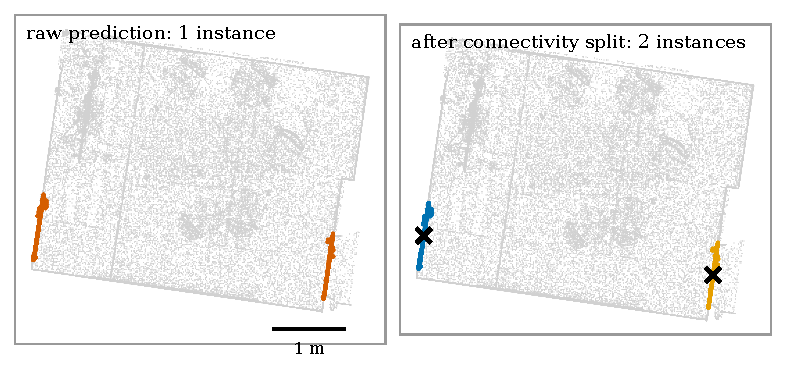
\includegraphics[width=\textwidth]{figs/fig_split_before_after}
\caption{\textbf{Structural splitting, validation scene
\texttt{5748ce6f01}.} Left: the model merges two distant, visually similar
door leaves --- on opposite walls, $4.2$\,m apart --- into one predicted
instance, so merging is a structural defect of the model, not a proximity
artifact. Right: DBSCAN $\varepsilon$-connectivity separates the mask into
its two spatial components ($5267$ and $5295$ points; centroids marked),
and every downstream geometric quantity is then computed per leaf.}
\label{fig:split}
\end{figure}

The model routinely merges the two leaves of a double door --- or two
adjacent handles --- into a \emph{single} predicted instance
(Figure~\ref{fig:split}). The direct cost is familiar: against either
ground-truth instance the merged mask has IoU $\approx 0.5$, so both
matches sit at the metric's threshold and usually fall below it. The
indirect cost is worse and specific to our pipeline: every geometric prior
of \S\ref{sec:geo} is computed \emph{on the mask}, so a merged mask's PCA
axis runs diagonally across the pair and its ``perpendicular endpoint''
lands in the gap between the doors. A merged instance does not merely lose
its own point; it poisons the axis and origin that the whole method reads
off the geometry.

\subsection{The DBSCAN trio: split, filter, suppress}

The fix is offline connected-component splitting. Run DBSCAN
(\texttt{min\_samples}$=1$, so it is pure $\varepsilon$-connectivity) on the
points of each predicted mask, emit each spatial component as its own
instance, drop components below a minimum size, and finish with IoU-based
NMS to remove duplicates. We call this three-step post-process the
\emph{trio}. It runs on the dumped predictions plus the preprocessed point
coordinates --- no GPU, no re-inference.

For the movable task ($\varepsilon = 0.2$\,m, minimum $50$ points) the trio
raises validation mask \apfifty{} $0.5716 \to 0.5801$ and, rerunning the
geometric stack on the split masks, the joint metric $0.4621 \to 0.5021$;
on the test server, $0.3385 \to 0.3689$ (Figure~\ref{fig:progression}). As
the mechanism predicts, the gain concentrates in the origin term
($0.3601 \to 0.3955$): each leaf's PCA axis and endpoint origin are finally
computed on the right geometry. For the interaction task
($\varepsilon = 0.075$, minimum $5$ points, NMS at IoU $0.75$), validation
goes $0.5363 \to 0.6054$ and test $0.2686 \to 0.2864$.

Splitting is the extreme case of the parameter-free regime
(\S\ref{sec:geo}): ``two doors are two objects'' is not a fact about the
validation split, so there is no fitted optimism to give back. On the
movable task the transfer was indeed near-full (Figure~\ref{fig:transfer}).
On the interaction task the same trio realised $+0.069 \to +0.018$; the
absolute levels there differ by a factor of two ($0.54$ validation vs.\
$0.27$ test), and \S\ref{sec:extension}'s memorization finding
retroactively explains part of that gap --- we report the delta ratio as
measured.

\subsection{Per-class $\varepsilon$: cluster radius is element scale}

A single $\varepsilon$ for the interaction task is a compromise across
element sizes: handles are elongated, knobs and buttons are tiny. Splitting
the radius by class --- $\varepsilon = 0.1$ for handles (class 1),
$\varepsilon = 0.065$ for knobs/buttons (class 2) --- is one number per
physical scale. It lifts validation $0.6054 \to 0.6253$ and test
$0.2864 \to 0.2886$.

\subsection{Cleaning the handle source}

The hinge-side rule of \S\ref{sec:geo}(iii) consumes \emph{predicted} handle
masks, and those predictions carry the same merged-instance disease, so we
feed the movable pipeline the trio-processed interaction predictions
instead. Validation joint metric moves $0.5021 \to 0.5038$ (origin
$0.5393 \to 0.5411$); on test, $0.3689 \to \mathbf{0.3760}$ (origin
$0.3955 \to 0.4026$) --- an over-delivery relative to the validation
estimate, and our best pre-extension movable-test score. The two tasks are
coupled:
interaction post-processing quality is an input to movable origin
accuracy.

\subsection{A quota-timing mistake}

One episode from the original deadline day is worth recording as a negative
result about \emph{process}. Each test leaderboard allows one submission per
day. We spent the interaction-test slot at dawn on the per-class variant
($0.2886$). By dusk we had built a better candidate and no quota left to
submit it, and a competitor's buzzer submission took first place at
$0.2904$. The $0.0018$ deficit was not a modelling gap but a scheduling one.
On a deadline day the daily submission is the day's scarcest asset, and it
should be spent at the \emph{end} of the day, on the best artifact the day
produced.

\section{The Extension Window: Betting Against a Memorized Validation Set}
\label{sec:extension}

This section covers the final stage: a bet that the validation set
systematically hides generalization gains, and the finetune-plus-ensemble
that won the interaction task.

The campaign should have ended there, second on one board of four. It did
not: server outages led the organizers to extend the deadline by roughly
24 hours, refreshing the daily submission quotas. That gave us something we
had never had --- a test-verification window --- and we spent it on a
hypothesis that had been unfalsifiable all month.

\subsection{The bet}

The released interaction checkpoint was trained on train$+$validation
(\S\ref{sec:data}; \S\ref{sec:originhead} already noted the movable analogue
inflates validation by $\sim$$0.01$). Its validation score of $0.536$ is
therefore an \emph{in-sample} number: the model has seen those scenes. Any
finetune we produce is scored \emph{out-of-sample} on that same split, so
validation systematically underrates finetunes relative to the baseline.
The only honest arbiter is the test server, and until the extension we
never had the quota to use it as one.

Why bet on augmentation specifically? Three earlier measurements pointed the
same way. The released training configuration has geometric augmentation
disabled entirely (and the repository's flip-time axis-label transform
contains a sign bug, which we fixed). Mirrored scenes are
out-of-distribution for the released backbone (recall $55.9\%$ vs.\
$70.5\%$, \S\ref{sec:negative}). And our own val$\to$test transfer at
$\sim$$1{:}3$ had the smell of a generalization deficit. A model that has
never seen a flipped scene, evaluated on a split it memorized, is exactly
the setting in which an augmentation dividend would be real and invisible.

\subsection{\texttt{v5}: the flips-only finetune}

\texttt{v5} finetunes the released interaction checkpoint on
train$+$validation with mirror-flip augmentation, coarse-to-fine curriculum
\emph{off} (\S\ref{sec:c2f}), learning rate $10^{-5}$, $60$ epochs, batch
size $1$, cropping on. In-sample validation moved by $+0.004$ only
($0.536 \to 0.540$). On test it moved by $+0.027$:
$0.2886 \to \mathbf{0.3156}$. This is the single deepest observation of the
campaign, and the $\sim$$700\%$ bar of Figure~\ref{fig:transfer}: the
augmentation dividend is nearly invisible on a memorized validation set,
because what it buys is precisely the generalization that in-sample
evaluation cannot see. Had we trusted validation, \texttt{v5} would have
been discarded as a wash.

\subsection{\texttt{v6} and the equal-strength ensemble}

\texttt{v6} repeats the recipe with random yaw rotation added. Solo it is
weaker ($0.529$ validation) --- but its augmentation spectrum differs from
\texttt{v5}'s, which is the property an ensemble needs. We take the union of
\texttt{v5} and \texttt{v6} proposals, then run the per-class DBSCAN trio
over the union with NMS at $0.55$: validation $0.6446$, test
$\mathbf{0.3240}$ --- first place at the time, $0.034$ clear of the
then-visible runner-up's $0.2904$.

We had tried proposal-union ensembling before and it failed: a union of the
baseline with a weaker finetune scored \emph{below} the baseline's own
post-processed validation score ($0.587$ vs.\ $0.605$) --- the weak member's
proposals dilute the strong member's ranking. The boundary condition the
two experiments bracket: proposal-union ensembling works when members are
near-equal in strength and diverse in training distortion, not otherwise.

\subsection{The coarse-to-fine trap: curriculum state is part of the
checkpoint}
\label{sec:c2f}

The most destructive pitfall of the campaign hides in the training schedule,
not the weights. The repository's coarse-to-fine curriculum dilates the
target masks by a radius $r \cdot \gamma^{\lfloor e/\alpha \rfloor}$ with
$r = 0.1$\,m and $\alpha = 100$: for the first $100$ epochs of \emph{any}
run, supervision is masks inflated by $10$\,cm. The released checkpoints
were trained through the whole curriculum (dilation decayed to zero). A
finetune launched from them with the curriculum enabled therefore
\emph{restarts} it, and spends its entire budget re-teaching the model to
predict dilated masks.

This destroyed two runs before we found it. An interaction finetune
collapsed $0.536 \to 0.008$ in \apfifty{} while AP$_{25}$ survived at $0.20$
--- the fingerprint of masks that are right but fat. A movable full-network
retrain jumped in score exactly when the first decay triggered at epoch
$100$. A hybrid experiment (finetuned weights, baseline BatchNorm buffers)
ruled out BN drift as the cause. Until the mechanism was found, these
collapses had us concluding that ``retraining hurts'' --- a wrong lesson
drawn from a confounded experiment, and the reason the bet of this section
was almost never placed. The general statement: \emph{curriculum state is
part of the checkpoint}. Finetuning must disable, or fast-forward, every
schedule-dependent transform of the training targets.

\subsection{Negative results of the extension window}

The window also funded a burst of cheap experiments, most of which failed
informatively; the bottom block of Table~\ref{tab:negative} lists them. One
deserves prose. \texttt{v10}, a movable full-network retrain with the
curriculum correctly disabled, reached mask \apfifty{} $0.404$ at epoch
$184$ against the released $0.572$: fixing the trap of \S\ref{sec:c2f} was
necessary but not sufficient on the movable side. The released weights
carry an official $1160{+}680$-epoch schedule, and $195$ scenes at batch
size $1$ on a single 24\,GB GPU do not close that gap in a day. The
curriculum explains the interaction collapse; compute explains the movable
one.

\subsection{Final standings}

\begin{table}[t]
\centering
\small
\begin{tabular}{lcccc}
\toprule
Leaderboard (ranking metric) & ours & \texttt{TnG} & \texttt{teamzb} & margin \\
\midrule
movable dev (\metric{})       & \textbf{0.5038} & --- & 0.4434 & $+0.0604$ \\
movable test (\metric{})      & 0.4056 & \textbf{0.4828} & 0.3711 & $-0.0772$ \\
interaction dev (\apfifty{})  & \textbf{0.6446} & --- & 0.6394 & $+0.0052$ \\
interaction test (\apfifty{}) & 0.3286 & \textbf{0.3446} & 0.3110 & $-0.0160$ \\
\bottomrule
\end{tabular}
\caption{\textbf{Final leaderboards} (2026-08-28): first on both dev boards, second on both
test boards. Margin is ours minus the best other entry. Our final movable
test sub-metrics: \apfifty{} $0.4668$, AP$_{50}^{\text{axis}}$ $0.4315$,
AP$_{50}^{\text{origin}}$ $0.4328$.}
\label{tab:final}
\end{table}

Table~\ref{tab:final} gives the final standings. The run in flight
delivered: \texttt{mov\_v11} --- the \texttt{v5} recipe transplanted to the
movable model (train$+$validation, flips only, curriculum off, learning
rate $10^{-5}$, $60$ epochs) --- raised in-sample validation mask
\apfifty{} from $0.5716$ to $0.5911$ raw ($0.6259$ after splitting) and
full-pipeline validation joint to $0.5319$; on test, joint
$\mathbf{0.4056}$ with \apfifty{} $0.4668$ (from $0.4444$; axis $0.4315$,
origin $0.4328$), against $0.3760$ before it. The augmentation dividend
transplanted to the movable model and over-delivered again. On the
interaction side, a three-model ensemble (\texttt{v5}$+$\texttt{v6}$+$%
\texttt{v5b}; validation $0.6513$) reached test $\mathbf{0.3286}$, our
final score there.

The final hours also redrew the boards: competitors who had kept their
submissions private all month went public at the buzzer, and \texttt{TnG}
took both test boards ($0.4828$ movable, $0.3446$ interaction). Scores at
that level indicate a fully retrained segmentation model, consistent with
our own finding that mask quality is the sole remaining bottleneck
(\S\ref{sec:collapse}). We finished first on both dev leaderboards and
second on both test leaderboards.

\section{Lessons}

We close with the campaign's transferable lessons, each tied to the
experiment that taught it.

\begin{enumerate}
\item \textbf{Diagnose before training --- and re-diagnose after every
  change.} Every effective component traces to a specific, quantified
  failure mechanism; both expensive failures (v4 collapse, BN drift) came
  from acting before measuring. Worse, we kept optimising against a
  \emph{stale} diagnosis --- days of lateral-hinge work read a map of the
  baseline's errors, not the deployed pipeline's; ten minutes of
  re-measurement (\S\ref{sec:sweep}) found more.
\item \textbf{Freezing parameters does not freeze behavior.} Buffers
  (BatchNorm statistics) update in training mode regardless of
  \texttt{requires\_grad}; verify claims of ``frozen'' by diffing
  checkpoints end-to-end.
\item \textbf{Match the loss to the metric.} Sign-agnostic axis loss
  ($1-|\cos|$), point-to-line origin loss, and axis normalization at
  submission time each exist because the evaluator says so.
\item \textbf{Geometry transfers; tuned thresholds do not.} The val$\to$test
  transfer ratio was $\sim$$3\times$ higher for parameter-free geometric
  rules than for validation-fitted post-processing. The practical test is
  not whether a threshold has an optimum but whether it has a
  \emph{plateau}, and stating a rule as a relation between two parts
  instead of a property of one made the whole swept range safe
  (\S\ref{sec:geo}) --- a stronger physical claim buys robustness that no
  amount of threshold tuning can.
\item \textbf{An oracle proves existence, not reachability.} The predicted
  mask always contains a point $6$\,mm from the true hinge line, so origin's
  ceiling is $100\%$ --- and we briefly concluded that post-processing would
  suffice. Four subsequent methods failed to select that point. An oracle
  measures the representation, not whether any available signal can pick
  the right element out of it; report the two separately.
\item \textbf{A negative result needs power to mean anything.} We cited a
  seven-positive probe as proof that the backbone lacks lateral-hinge
  information, and let it close a research direction for days. The properly
  powered version agrees, which is luck, not method: with seven positives an
  AUC cannot distinguish absence from noise. Before retiring a direction on
  an against-the-null result, check that the null had something to reject.
\item \textbf{Measure a representation's ceiling before building on it.}
  This is the same discipline as the previous point, applied forwards. We
  ran the superpoint intervention first and the ceiling analysis after, and
  the ceiling turned out to be \emph{below} what we already had.
\item \textbf{Optimise the metric you are scored on, not a proxy for it.}
  Per-instance retention and AP disagree in sign: taking the panel normal
  unconditionally raises matched-instance retention from $91.6\%$ to
  $96.8\%$ while \emph{lowering} AP$_{50}^{\text{axis}}$ by $0.010$, because
  retention sees only confident, well-matched instances and AP integrates
  the low-confidence tail where the same geometry is unreliable. Diagnostics
  that restrict to the easy subset will recommend changes that lose.
\item \textbf{Validate the oracle, not just the model.} An upper bound is a
  measurement of the \emph{evaluator} as much as of the method. On this
  benchmark the ideal oracle scores $0.65$, not $1.0$, because bit-exact
  axes trigger an $\arccos$ domain overflow (\S\ref{sec:oracle-artifact});
  any headroom estimate that assumes an oracle reaches $1.0$ is wrong by a
  third, and the error is concentrated on exactly the sub-task the method
  targets.
\item \textbf{Leaderboard forensics is a research tool.} Retention-rate
  analysis of competitors' four public numbers correctly predicted that the
  leader's advantage was geometric rather than architectural, and pointed to
  the exact sub-tasks (translation azimuth, hinge side) where the gap lay.
\item \textbf{Structural fixes transfer near-fully; tuned thresholds tithe.}
  Our final taxonomy of val$\to$test transfer has three regimes:
  validation-tuned thresholds realise $\sim$$1/3$ of their gain;
  physically-correct rules realise it in proportion to how often they fire
  on the target split; and structural fixes --- repairs of
  distribution-independent defects like a merged double door --- transfer
  near-fully ($+0.040 \to +0.030$ for the DBSCAN split,
  \S\ref{sec:structural}). Budget submissions accordingly.
\item \textbf{A memorized validation set hides exactly the gains that
  matter.} A checkpoint trained on train$+$validation makes validation an
  in-sample score, and the generalization that augmentation buys is then
  nearly invisible there ($+0.004$ val vs.\ $+0.027$ test for \texttt{v5},
  \S\ref{sec:extension}). When quota permits, insist on held-out arbitration
  before discarding a finetune that validation calls a wash.
\item \textbf{Proposal-union ensembling has a boundary condition.} It worked
  with two near-equal, differently-augmented finetunes ($0.3240$ on test)
  and failed with a strong--weak pair ($0.587$ vs.\ $0.605$ on validation):
  the union of unequal members dilutes the stronger one. Check member parity
  before spending an ensemble submission.
\item \textbf{Curriculum state is part of the checkpoint.}
  Schedule-dependent target transforms (here, coarse-to-fine mask dilation
  restarting at $r=0.1$\,m, $\alpha=100$) silently reset when finetuning
  resumes at epoch zero, and destroyed two runs ($0.536 \to 0.008$) before
  being identified (\S\ref{sec:c2f}). Worse than the lost runs was the lost
  conclusion: the collapses read as ``retraining hurts'' and nearly buried
  the campaign's most profitable bet.
\item \textbf{On deadline days, spend the daily quota at the end of the
  day.} We submitted at dawn, improved by dusk, and were overtaken by a
  buzzer submission ($0.2904$ vs.\ our $0.2886$); the $0.0018$ was a
  scheduling gap, not a modelling one (\S\ref{sec:structural}).
\end{enumerate}

\section{Conclusion}

A reproduced USDNet baseline ($0.264$ test \metric{}) reaches $0.4056$ ---
$+54\%$ relative, first on both dev leaderboards and second on both test
leaderboards --- in three stages (Figure~\ref{fig:progression}): one tiny
trained head plus training-free geometric priors ($0.264 \to 0.3385$,
$+28\%$ relative); an offline structural split of merged instances
(\S\ref{sec:structural}); and an extension-window bet --- augmented
finetunes and ensembles on both tasks --- that delivered the final scores
($\to 0.4056$; interaction $0.2686 \to 0.3286$, $+22\%$,
\S\ref{sec:extension}). The segmentation branch stayed frozen through the
first two stages, with one deliberate, offline exception: splitting what
the model had merged.

The deepest single observation belongs to the last stage. A released
checkpoint trained on validation makes validation nearly blind to
generalization gains --- our mirror-flip finetune moved the memorized split
by $+0.004$ and the test set by $+0.027$ --- so held-out arbitration is
worth paying submission quota for. The axis head's total collapse onto
gravity remains unsolved: it emits $[0,0,1]$ for $95.6\%$ of rotations and
is wrong on the rest, ten interventions failed to recover the lateral
hinges, and the $\mathbb{RP}^2$ treatment sketched in \S\ref{sec:collapse}
is still the one untested idea aimed at the mechanism rather than the
symptom. We hope the more than two dozen documented negative results, the
freezing, curriculum and evaluation pitfalls, and the confounded-submission
postmortems of \S\ref{sec:confound} and \S\ref{sec:c2f} are as useful as the
recipe itself.

\paragraph{Acknowledgments.} Based on the USDNet/Articulate3D toolkit and the
ScanNet++ dataset; we thank the challenge organizers.

\bibliographystyle{plain}
\bibliography{refs}

\end{document}
